\chapter{TacOSのメッセージ通信}
\label{tacosIPC}
TacOSではマイクロカーネルがメッセージ通信機構を提供し,
ユーザ・プロセスとサーバプロセス,
サーバプロセスとサーバプロセスの通信にメッセージを用いる.

%==============================================================================
\section{メッセージ通信機構}
TacOSのメッセージ通信機構は,
クライアントプロセスがサーバプロセスの機能を利用する,
クライアント・サーバの通信に特化したランデブー方式である.
\figref{tacosMessage}にTacOSのメッセージ通信の様子を示す.
メッセージ通信の手順は次のようになる.

\begin{myfig}{btp}{TacOSのメッセージ通信}{tacosMessage}
  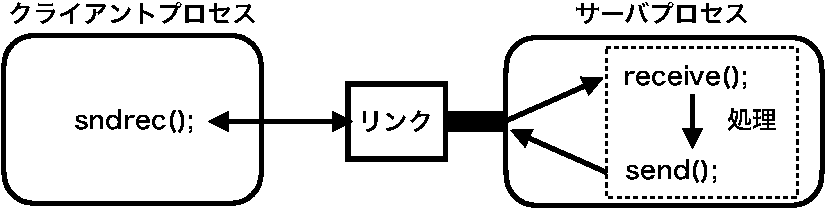
\includegraphics[scale=0.75]{Fig/tacosMessage-crop.pdf}
\end{myfig}

\begin{enumerate}
\item サーバプロセスが\emph{リンク}を所有し他プロセスからの通信を待ち受ける.
\item クライアントプロセスは
  \|sndrec()|関数を用いてリンクに処理内容をメッセージとして送信する.
  \item サーバプロセスは\|receive()|関数を用いてメッセージを受信する.
  \item サーバプロセスはメッセージの内容に合った処理を行う.
  \item サーバプロセスは処理結果を\|send()|関数を用いて返信する.
  \item \|sndrec()|関数が完了し,クライアントプロセスは処理結果を受取る.
\end{enumerate}

TacOSのメッセージ通信機構は,
\emph{間接指定方式},\emph{固定長},\emph{ランデブー方式}と言える.
クライアントプロセスとサーバプロセスが並列に処理することができないが,
%マイクロカーネル方式であるので
サービスモジュールをサーバプロセスにすることができ,
オペレーティングシステムを構築するためのプログラミングを容易にしている.

%==============================================================================
\section{リンク構造体}
リスト\ref{tacosLink}にリンク構造体の宣言を示す\footnote{
  \url{https://github.com/tctsigemura/TacOS/blob/master/os/kernel/process.hmm}
  の一部である.}.
\|Link|構造体はランデブー用のリンクを定義している.
\|server|はリンクを所有するサーバプロセスのPCB,
\|client|はリンクを使用中のクライアントプロセスのPCBである.
\|s1|,\|s2|,\|s3|は
相互排除と同期のために使用されるセマフォである.
TacOSのリンクはセマフォを基盤にしている.
\|op|,\|prm1|,\|prm2|,\|prm3|が固定長のメッセージ本体になる.

\lstinputlisting[numbers=left,float=btp,label=tacosLink,
  firstline=107,lastline=119,
  caption=TacOSのリンク構造体]{TacOS/kernel/process.hmm}

%==============================================================================
\section{リンクの作成}
リスト\ref{tacosNewLink}に,
TacOSのマイクロカーネル内のリンク作成ルーチンを示す\footnote{
  \url{https://github.com/tctsigemura/TacOS/blob/master/os/kernel/kernel.cmm}の
  一部である.}.
\|newLink()|関数はサーバプロセスがリンクを作り所有するために呼び出す.
TacOSのサーバプロセスはカーネルモードで実行され,
マイクロカーネル内ルーチンを呼び出すことができる.
複数のプロセスが\|newLink()|関数を呼び出す可能性があるので,
6行から19行の範囲は割込み禁止による相互排除を行っている.

\lstinputlisting[numbers=left,float=btp,label=tacosNewLink,
  firstline=496,lastline=516,
  caption=TacOSのリンク作成ルーチン]{TacOS/kernel/kernel.cmm}

空きリンクは7行で管理している.
リンクの廃棄手段は準備されていないので,
空きリンクの管理は単純である.
15行でリンクを所有するサーバプロセスを記録する.
16,17,18行で,三つのセマフォをリンクに割当てている.
20行では作成したリンクの番号を返している.

%==============================================================================
\section{サーバ用のメッセージ通信ルーチン}
マイクロカーネル内にある,
サーバプロセス用のメッセージ通信プログラムを
リスト\ref{tacosSendReceive}に示す\footnote{
  \url{https://github.com/tctsigemura/TacOS/blob/master/os/kernel/kernel.cmm}
  の一部である.}.
2行の\|receive()|関数はメッセージの受信に使用する.
引数\|num|は\|newLink()|が返したリンク番号である.
4行でリンクの所有者を調べている.
所有者が自身ではないならオペレーティングシステムのバグなので
\|panic()|関数を用いてシステムを停止する.
5行で初期値0のセマフォ(\|s1|)にP操作を行い,
クライアントがリンクにデータを書き込むのを待つ.
6行でデータが書き込まれたリンクを返す.

\lstinputlisting[numbers=left,float=btp,label=tacosSendReceive,
  caption=TacOSのメッセージ通信ルーチン(サーバ用),
  firstline=518,lastline=532]{TacOS/kernel/kernel.cmm}

10行の\|send()|関数は,
クライアントプロセスにメッセージを返信するために使用する.
引数\|num|はリンク番号,\|res|は返信するデータである.
サーバが行った処理の結果を16ビット(2バイト)で表現する.
12行では\|receive()|関数と同様にリンクの所有者を調べている.
13行で処理結果をリンクに書込み,
14行でクライアントが待ち合わせているセマフォ(\|s3|)にV操作を行う.
これでクライアントが処理結果を受取り処理を再開する.

%==============================================================================
\section{サーバプロセスの例}
リスト\ref{tacosPmMain}にサーバプロセスの例として,
プロセスマネージャのメインルーチンを示す\footnote{
  \url{https://github.com/tctsigemura/TacOS/blob/master/os/pm/pm.cmm}の
  一部である.}.
プロセスマネージャはexecシステムコール等を処理するサーバプロセスである.
3行でリンクを作成し\|pmLink|グローバル変数\footnote{
  \url{https://github.com/tctsigemura/TacOS/blob/master/os/pm/pm.hmm}
  で宣言されている.}に記録する.
5行でクライアントプロセスからのメッセージを待ち受ける.
メッセージを受信したら6行に進み,
リンクに書き込まれていた内容とクライアントプロセスのPCBを引数に,
プロセスマネージャのシステムコール処理ルーチンを実行する.
処理結果は7行の\|send()|関数を用いてクライアントプロセスに返信する.

\lstinputlisting[numbers=left,float=btp,label=tacosPmMain,
  caption=TacOSのメッセージ通信使用例(サーバ側),
  firstline=286,lastline=294]{TacOS/pm/pm.cmm}

%==============================================================================
\section{クライアント用のメッセージ通信ルーチン}
リスト\ref{tacosSndRec}にTacOSのクライアントプロセス用の
メッセージ通信プログラム(\|sndrec()|)を示す\footnote{
  \url{https://github.com/tctsigemura/TacOS/blob/master/os/kernel/kernel.cmm}の
  一部である.}.
\|sndrec()|関数はサーバプロセスのリンクにメッセージを書込み,
サーバプロセスに処理を依頼する.
サーバプロセスが処理を完了したら,
\|sendrec()|関数は処理結果を返り値として終了する.

\lstinputlisting[numbers=left,float=btp,label=tacosSndRec,
  caption=TacOSのメッセージ通信ルーチン(クライアント用),
  firstline=534,lastline=550]{TacOS/kernel/kernel.cmm}

4行では初期値1のセマフォ(\|s2|)を用いてリンクをロックし,
他のクライアントプロセスとの相互排除を行っている.
6行から9行でリンクにメッセージを書き込む.
\|iSemV()|関数を使用するために,
10行から13行まで割込み禁止による相互排除を行っている.
11行でメッセージを書き込んだことをサーバに知らせ,
12行で初期値0のセマフォ(\|s3|)にP操作を行いサーバが処理を終了するのを待つ.
サーバの処理が終了したら14行に進み
サーバがリンクに書き込んだ処理結果を取り出す.
15行でリンクのロックを解除し16行で処理結果を持って関数を終了する.

%==============================================================================
\section{クライアントプロセスの例}
リスト\ref{tacosPmExec}にメッセージ通信機構のクライアント側の例として,
プロセスマネージャ(サーバプロセス)に
execシステムコールの処理を依頼するプログラムを示す\footnote{
  \url{https://github.com/tctsigemura/TacOS/blob/master/os/pm/pm.cmm}の
  一部である.}.
TacOSのexecシステムコールは,
新しいプロセスを作ってプログラムを実行させる.
引数はプログラムファイルのパス名(\|path|)と,
新しいプログラムの\|main()|関数に渡すコマンド行引数(\|argv|)である.

\lstinputlisting[numbers=left,float=btp,label=tacosPmExec,
  caption=TacOSのメッセージ通信使用例(クライアント側),
  firstline=302,lastline=305]{TacOS/pm/pm.cmm}

1行はクライアントプロセスのexecシステコールの入口になる.
カーネルモードで動作する他のサーバプロセスは\|exec()|関数を直に呼び出す.
ユーザモードで動作するユーザプロセスはSVC機械語命令で割込みを発生し,
SVC割込みハンドラから\|exec()|関数を呼び出す.
割込みハンドラは現在のプロセスのコンテキストで実行されるので,
\|exec()|関数はカーネルモードに切り換わった状態の
ユーザプロセスによって実行されることになる.

2行でプロセスマネージャ(サーバプロセス)とランデブーを行う.
\|pmLink|はリスト\ref{tacosPmMain}で
プロセスマネージャが生成したリンクである.
\|EXEC|がシステムコールの種類を表している.
システムコールの二つの引数は\|_AtoI()|関数を用いてint型に変換して渡している.
処理結果は子プロセスのプロセス番号(PID)である.
3行でPIDを呼び出し側に返す.

%==============================================================================
\section{まとめ}
TacOSのメッセージ通信について,
それを実現するマイクロカーネル内プログラムと利用例を示した.

%==============================================================================
\section*{練習問題}
\begin{enumerate}
  \renewcommand{\labelenumi}{\ttfamily\arabic{chapter}.\arabic{enumi}}
  \setlength{\leftskip}{1em}
\item TacOSのメッセージ通信機構について正しいか正しくないか答えなさい.
  \begin{enumerate}
  \item メッセージの形式に柔軟性がある.
  \item リンクに三つのセマフォが含まれる.
  \item TacOSのメッセージ通信機構は相互排除と同期にセマフォだけを用いている.
  \item 複数生産者と複数消費者の問題の解に使用できる.
  \end{enumerate}
\end{enumerate}
